\def\year{2021}\relax
%File: formatting-instructions-latex-2021.tex
%release 2021.1
\documentclass[letterpaper]{article} % DO NOT CHANGE THIS
\usepackage{aaai21}  % DO NOT CHANGE THIS
\usepackage{times}  % DO NOT CHANGE THIS
\usepackage{helvet} % DO NOT CHANGE THIS
\usepackage{courier}  % DO NOT CHANGE THIS
\usepackage[hyphens]{url}  % DO NOT CHANGE THIS
\usepackage{graphicx} % DO NOT CHANGE THIS
\usepackage{subfigure}
\urlstyle{rm} % DO NOT CHANGE THIS
\def\UrlFont{\rm}  % DO NOT CHANGE THIS
\usepackage{natbib}  % DO NOT CHANGE THIS AND DO NOT ADD ANY OPTIONS TO IT
\usepackage{caption} % DO NOT CHANGE THIS AND DO NOT ADD ANY OPTIONS TO IT
\frenchspacing  % DO NOT CHANGE THIS
\setlength{\pdfpagewidth}{8.5in}  % DO NOT CHANGE THIS
\setlength{\pdfpageheight}{11in}  % DO NOT CHANGE THIS
%\nocopyright
%PDF Info Is REQUIRED.
% For /Author, add all authors within the parentheses, separated by commas. No accents or commands.
% For /Title, add Title in Mixed Case. No accents or commands. Retain the parentheses.
\pdfinfo{
%/Title (Generalized Out-of-distribution Indicator via Deep Generative Models)
%/Author (Wenxiao Chen, Xiaohui Nie, Mingliang Li, Dan Pei)
%/TemplateVersion (2021.1)
} %Leave this
% /Title ()
% Put your actual complete title (no codes, scripts, shortcuts, or LaTeX commands) within the parentheses in mixed case
% Leave the space between \Title and the `ning parenthesis alone
% /Author ()
% Put your actual complete list of authors (no codes, scripts, shortcuts, or LaTeX commands) within the parentheses in mixed case.
% Each author should be only by a comma. If the name contains accents, remove them. If there are any LaTeX commands,
% remove them.

% DISALLOWED PACKAGES
% \usepackage{authblk} -- This package is specifically forbidden
% \usepackage{balance} -- This package is specifically forbidden
% \usepackage{color (if used in text)
% \usepackage{CJK} -- This package is specifically forbidden
% \usepackage{float} -- This package is specifically forbidden
% \usepackage{flushend} -- This package is specifically forbidden
% \usepackage{fontenc} -- This package is specifically forbidden
% \usepackage{fullpage} -- This package is specifically forbidden
% \usepackage{geometry} -- This package is specifically forbidden
% \usepackage{grffile} -- This package is specifically forbidden
% \usepackage{hyperref} -- This package is specifically forbidden
% \usepackage{navigator} -- This package is specifically forbidden
% (or any other package that embeds links such as navigator or hyperref)
% \indentfirst} -- This package is specifically forbidden
% \layout} -- This package is specifically forbidden
% \multicol} -- This package is specifically forbidden
% \nameref} -- This package is specifically forbidden
% \usepackage{savetrees} -- This package is specifically forbidden
% \usepackage{setspace} -- This package is specifically forbidden
% \usepackage{stfloats} -- This package is specifically forbidden
% \usepackage{tabu} -- This package is specifically forbidden
% \usepackage{titlesec} -- This package is specifically forbidden
% \usepackage{tocbibind} -- This package is specifically forbidden
% \usepackage{ulem} -- This package is specifically forbidden
% \usepackage{wrapfig} -- This package is specifically forbidden
% DISALLOWED COMMANDS
% \nocopyright -- Your paper will not be published if you use this command
% \addtolength -- This command may not be used
% \balance -- This command may not be used
% \baselinestretch -- Your paper will not be published if you use this command
% \clearpage -- No page breaks of any kind may be used for the final version of your paper
% \columnsep -- This command may not be used
% \newpage -- No page breaks of any kind may be used for the final version of your paper
% \pagebreak -- No page breaks of any kind may be used for the final version of your paperr
% \pagestyle -- This command may not be used
% \tiny -- This is not an acceptable font size.
% \vspace{- -- No negative value may be used in proximity of a caption, figure, table, section, subsection, subsubsection, or reference
% \vskip{- -- No negative value may be used to alter spacing above or below a caption, figure, table, section, subsection, subsubsection, or reference

\usepackage{amsmath}
\usepackage{amssymb}
\usepackage{cleveref}
\usepackage{booktabs}
\usepackage[switch]{lineno}  %

\newtheorem{theorem}{Theorem}
\newtheorem{lemma}{Lemma}
\newtheorem{proof}{Proof}[section]

\newcommand{\IE}{\textit{i.e.}, }
\newcommand{\EG}{\textit{e.g.}, }
\newcommand{\ET}{\textit{et al.}}
\newcommand{\ST}{\textit{s.t.}}


\newcommand{\dd}{\mathrm{d}}
\newcommand{\vv}[1]{\bm{\mathrm{{#1}}}}
\newcommand{\E}{\operatorname{\mathbb{E}}}
\newcommand{\pin}{p_{in}}
\newcommand{\pout}{p_{out}}
\newcommand{\pmix}{p_{mix}}


\setcounter{secnumdepth}{1} %May be changed to 1 or 2 if section numbers are desired.

% The file aaai21.sty is the style file for AAAI Press
% proceedings, working notes, and technical reports.
%

% Title

% Your title must be in mixed case, not sentence case.
% That means all verbs (including short verbs like be, is, using,and go),
% nouns, adverbs, adjectives should be capitalized, including both words in hyphenated terms, while
% articles, conjunctions, and prepositions are lower case unless they
% directly follow a colon or long dash

\title{A Framework of Robust Out-of-Distribution Indicators \\ Based on Divergence in Deep Generative Models}
\author{
    %Authors
    % All authors must be in the same font size and format.
%    Wenxiao Chen, Xiaohui Nie, Mingliang Li, Dan Pei
}
\affiliations{
    %Afiliations

%    Department of Computer Science and Technology, Tsinghua University
%    China Unicom
	
    %If you have multiple authors and multiple affiliations
    % use superscripts in text and roman font to identify them.
    %For example,

    % Sunil Issar, \textsuperscript{\rm 2}
    % J. Scott Penberthy, \textsuperscript{\rm 3}
    % George Ferguson,\textsuperscript{\rm 4}
    % Hans Guesgen, \textsuperscript{\rm 5}.
    % Note that the comma should be placed BEFORE the superscript for optimum readability

    % email address must be in roman text type, not monospace or sans serif
%    chen-wx17@mails.tsinghua.edu.cn

    % See more examples next
}
\iffalse
%Example, Single Author, ->> remove \iffalse,\fi and place them surrounding AAAI title to use it
\title{My Publication Title --- Single Author}
\author {
    % Author
    Author Name \\
}

\affiliations{
    Affiliation \\
    Affiliation Line 2 \\
    name@example.com
}
\fi

\iffalse
%Example, Multiple Authors, ->> remove \iffalse,\fi and place them surrounding AAAI title to use it
\title{My Publication Title --- Multiple Authors}
\author {
    % Authors

        First Author Name,\textsuperscript{\rm 1}
        Second Author Name, \textsuperscript{\rm 2}
        Third Author Name \textsuperscript{\rm 1} \\
}
\affiliations {
    % Affiliations
    \textsuperscript{\rm 1} Affiliation 1 \\
    \textsuperscript{\rm 2} Affiliation 2 \\
    firstAuthor@affiliation1.com, secondAuthor@affilation2.com, thirdAuthor@affiliation1.com
}
\fi
\begin{document}
\linenumbers  %

\maketitle

\begin{abstract}

Currently, deep generative models are widely researched in detecting out-of-distribution (OoD) problem. We reviewed the recent researches about out-of-distribution based on deep generative models and found one critical weakness that the number of datasets in these works is not enough to support the generality of their indicators. 
Therefore, we do large-scale research for these indicators on more datasets and find that these indicators on common deep generative models do not perform well on large-scale datasets. 
Here we propose the KL-based indicator and Wasserstein-based indicator for detecting out-of-distribution. 
Our indicators are general with solid theoretical inference and proven to be better than traditional indicators. They are expected to guide the development of deep generative models in the OoD domain. 
Our indicators outperform past works by 10\% in AUROC and their performance is near to theoretical optimal result. Moreover, our systematic experiments show that our indicators are not data-specific and can be deployed online. 
 
\end{abstract}

\section{Introduction}
Machine learning has achieved impressive success in the classification domain through deep neural network classifiers~\cite{szegedy2016inception,he2016deep,zagoruyko2016wide}. However, these classifiers can be easily fooled to provide with high confidence when the training and testing distribution differ (called in-distribution and out-of-distribution, OoD)~\cite{nguyen2015deep}, which might lead to potential risks in practice. 
For example, a classifier trained on CIFAR-10~\cite{krizhevsky2009learning} may recognize the house number in SVHN~\cite{netzer2011reading} as a horse. 
Detecting OoD data is crucial to ensure that applications based on classifiers are robust and reliable. 
Ostensibly, it is intuitive to train a density model $p_\theta(x)$ to approximate the empirical distribution of training data, and refuse the sample $x$ when $p_\theta(x)$ is sufficiently low~\cite{bishop1994novelty}. 
Recently, deep generative models are quickly developed and have been able to generate realistic samples, which indicates that deep generative models assign high density to the samples of the training data, and density can be used for detecting out-of-distribution. 

However, contrary to popular belief, recent works~\cite{nalisnick2019do,choi2018waic,hendrycks2018deep} show that density estimates by deep generative models assign higher density to samples from out-of-distribution. This phenomenon occurs in CIFAR-10 (as in-distribution) vs SVHN (as out-of-distribution) for different likelihood-based models, while the data in CIFAR-10 and SVHN have significant different semantic. 

Alternative indicators based on likelihood have been proposed~\cite{serra2019input,song2017pixeldefend,choi2018waic,ren2019likelihood,song2019unsupervised,che2019deep} to alleviate the issue. However, datasets considered in these works are quite less, even only CIFAR-10 and SVHN. It is a natural question whether these indicators work well on large-scale datasets because a robust OoD detection method should detect samples from any out-of-distribution~\cite{chen2020robust}. In this paper, we do large-scale experiments for these indicators on 14 popular datasets, including MNIST, FASHION-MNIST, KMNIST, NOT-MNIST, Omniglot, CIFAR-10, CIFAR-100, TinyImagenet, SVHN, iSUN, CelebA, LSUN, Noise and Constant. These indicators on common models perform not well on large-scale datasets. Based on the observation, we argue that \textit{evaluation on the few datasets is unreliable and evaluation on large-scale datasets should be a common sense in the OoD domain}. 

Based on the experiments on large-scale datasets, we found a common phenomenon that \textit{$p_\theta$ has a higher density for samples from in-distribution and lower density for samples from out-of-distribution than $p_\omega$}, which is trained on the out-of-distribution. 
Based on this phenomenon and theoretical proof, we propose the KL-based indicator for likelihood-based models for OoD detection. Traditional likelihood indicator only serves for log-likelihood based models, however GANs, the most popular generative models, are not likelihood-based models. To cover more generative models, the Wasserstein-based indicator is proposed for WGAN (a popular version of GAN with more stable training) based on the same theoretical framework. 

Our indicators outperform past works by 10\% in AUROC and its performance is near to theoretical optimal result. Moreover, our systematic experiments show that our indicators are not data-specific and can be deployed online. 

The main contributions of this paper are in the following:
\begin{itemize}
	\item We do large-scale experiments for indicators of previous works on large-scale datasets and find that these indicators based on common models perform not well. We argue that the few datasets will cause unreliable evaluation, and the evaluation on large-scale datasets should be a common sense in the OoD domain. 
	\item We propose the KL-based indicator and Wasserstein-based indicator for detecting out-of-distribution through a new theoretical framework instead of the traditional likelihood assumption. It is a novel idea for guiding the indicators based on deep generative models. 
	\item KL-based indicator and Wasserstein-based indicator outperform past works by 10\% in AUROC and its performance is near to optimal. Moreover, our systematic experiments show that our indicators are not data-specific and can be deployed online. 
\end{itemize}

\section{Background}
Likelihood-based generative models are widely viewed to be robust to detect out-of-distribution samples by the model density intuitively. However, the densities of common likelihood-based models, \EG RealNVP~\cite{dinh2016density}, VAE~\cite{tomczak2018vae,takahashi2019variational} and PixelCNN~\cite{van2016conditional}, have been shown to be problematic for detecting out-of-distributions~\cite{nalisnick2019do}. These likelihood-based models assign higher likelihood for samples from SVHN (out-of-distribution) than samples from CIFAR-10 (in-distribution). 

To solve this problem, some researches proposed some variants of these models for detecting out-of-distribution~\cite{che2019deep} and some researches proposed improved indicator to replace log-likelihood on common models~\cite{serra2019input}. Common models are widely applied in images domain and variants are not. Moreover, evaluation on numerous variants on large-scale datasets is more expensive while common models are easy for training and many indicators can share one well-trained model. Furthermore, it is necessary to check the generality of indicators on common models. By the above motivations, this paper focuses on the indicators based on common models. 

\cite{song2017pixeldefend} considered using permutation tests statistics $T_{perm}(x)$ as the indicator to detect OoD. The rank of $p_\theta(x)$ in the training set is used as OoD indicators. Both low-likelihood and high-likelihood samples are identified as OoD. It is significantly useful to solve the counterexample of CIFAR-10 vs SVHN in \cite{nalisnick2019do}. 

\cite{choi2018waic} used Watanabe Akaike Information Criterion (WAIC) based on model ensembles.
\begin{equation}
	\text{WAIC}(x) = \mathbb{E}_{\theta} [\log p_\theta(x)] - \operatorname{Var}_{\theta} [\log p_\theta(x)]
\end{equation}

\cite{ren2019likelihood} proposed a likelihood ratio indicator for deep generative models. They proposed a background model $p_{\theta_0}(x)$ to capture the general background statistics and a likelihood ratio indicator $LLR(x)$ to capture the significance of the semantics compared to the background model. 
\begin{equation}
LLR(x) = \log p_\theta(x) - \log p_{\theta_0}(x)
\end{equation}

\cite{serra2019input} observed that input complexity excessively affects the generative models' likelihoods. Based on this observation, they proposed an estimation for input complexity $L(x)$, to derive a parameter-free OoD indicator $S(x)$:
\begin{equation}
	S(x) = -\log p_\theta(x) - L(x)
\end{equation}

\cite{song2019unsupervised} observed that generative models with batch normalization assign much lower likelihood to OoD samples than in-distribution samples. 
%Meanwhile, the corresponding log-likelihood decreases dramatically for OoD samples, but is relatively stable for in-distribution samples, as the ratio of test samples in a batch increases. 
Based on the insight, $T_{b, r_1, r_2}(x)$ is proposed for OoD detection. 

Some researches also proposed to use labels (for classification tasks) to solve OoD. 
\cite{che2019deep} proposed $p(x|y)$ for OoD detection. It uses conditional deep generative models to verify the predictions of classifier. \cite{alemi2018uncertainty} use VIB to model the bottleneck $I(Z;Y)-\beta I(Z;X)$ where $I$ is the mutual information. 
\cite{hendrycks2016baseline,hendrycks2018deep,hsu2020generalized,lee2018simple,lakshminarayanan2017simple} proposed some indictors based on classifier for detecting OoD. 

\section{Problem Statement}\label{sec2}

$\pin$ and $\pout$ denote two distinct data distributions defined on image space $\mathcal{X}$ where $\pin$ is called in-distribution and $\pout$ is called out-of-distribution. 
$\pmix$ denotes a mixture distribution $\pmix(x) = \alpha \pin(x) + \beta \pout(x)$ where $\alpha + \beta = 1$ and $\alpha, \beta > 0$. 
The samples from $\pmix$, are generated by $\pin$ or $\pout$ and \textit{we wonder which of them are generated by $\pin$ without knowing any information about $\pout$}. 

It is important to decide whether two datasets are distinct on large-scale datasets. Two datasets are \textbf{simply-classified} when a common classifier which is trained on the training data of two datasets for 2-class classification, \IE in-distribution as label 0 and OoD as label 1, can simply distinguish the testing data of the two datasets. If two dataset A, B are simply-classified, A vs B (A as in-distribution and B as out-of-distribution) will be an experiment. 

In this paper, we consider the problem of distinguishing the in-distribution and out-of-distribution on the common deep generative models, \IE VAE, PixelCNN, flow-based models and GANs. Large-scale common datasets are used to validate the generality of indicators, as shown in \Cref{sec6}. 

All common metrics including AUROC, AUPR, AP, FPR@TPR95 are considered in this paper. AUROC is selected as the major metric and other metrics are shown in appendix B. AUROC is a threshold-independent metric~\cite{davis2006relationship} and is widely used in the OoD domain. % A perfect detector can get AUROC score of 100\%. 

\section{Motivating Observations}\label{sec3}

\begin{figure}[t]
\centering
\subfigure[CIFAR-10 vs SVHN]{
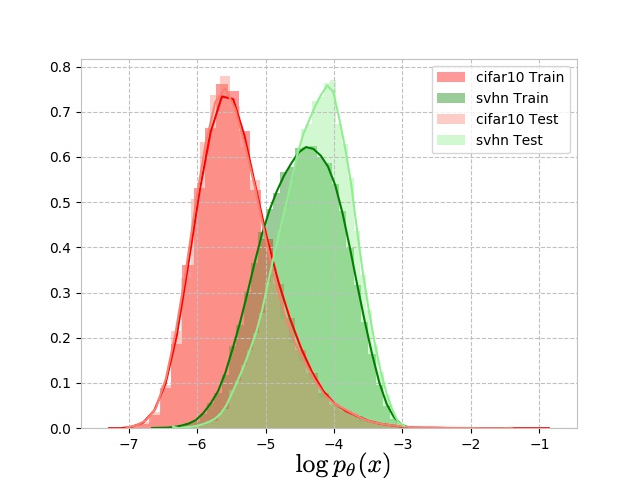
\includegraphics[width=0.45\columnwidth]{counterexample1.png}
}
\subfigure[KMNIST vs Omniglot]{
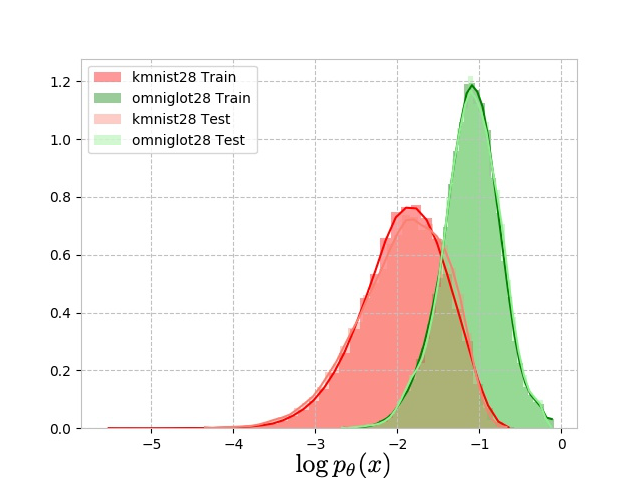
\includegraphics[width=0.45\columnwidth]{counterexample2.png}
}
\quad
\subfigure[SVHN vs CIFAR-10]{
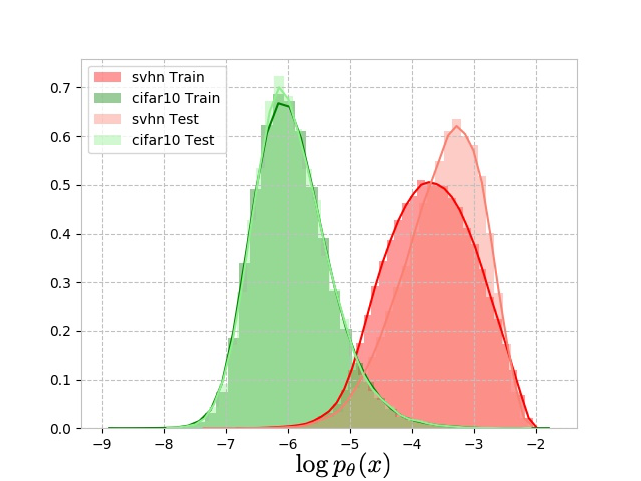
\includegraphics[width=0.45\columnwidth]{counterexample3.png}
}
\subfigure[MNIST vs Omniglot]{
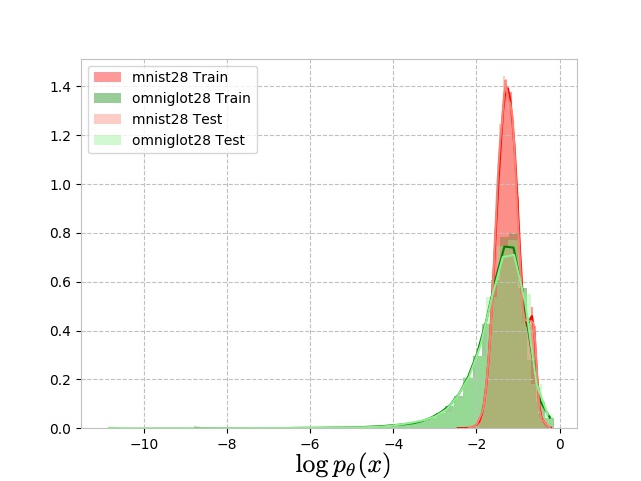
\includegraphics[width=0.45\columnwidth]{counterexample4.png}
}
\caption{The histogram of log-likelihood of VAE. 
% The value of log-likelihood is normalized by the size of images to BPD. 
Green and red parts denote the log-likelihood of out-of-distribution and in-distribution respectively. 
%Intuitively, we expect the log-likelihood of out-of-distribution are always higher than in-distribution. 
%However, these experiments show that log-likelihood of out-of-distribution might be higher, lower or nearly same to in-distribution. 
The AUROC of log-likelihood in (a) (b) (c) (d) are 0.08, 0.09, 0.99, 0.59. The AUROC of $T_{perm}$ in (a) (b) (c) (d) are 0.84, 0.82, 0.98, 0.66. }
\label{fig1}
\end{figure}

\subsection{Counterexamples}
Generally, the log-likelihood of likelihood-based models is expected to be lower in the out-of-distribution and be higher in the in-distribution intuitively because the models are trained on in-distribution. 
However, the observation of \cite{nalisnick2019do} shows that VAE, PixelCNN and RealNVP all assign the higher log-likelihood to samples from out-of-distribution in experiments CIFAR-10 vs SVHN and NotMNIST vs MNIST. 
We observed that the number of datasets in \cite{nalisnick2019do} is quite small and we suspect that there might be more counterexamples at large-scale datasets. 

Therefore, we reproduce the experiments at more datasets and find more counterexamples shown in \Cref{fig1} and appendix A. 
These experiments show that log-likelihood is unpredictable at out-of-distribution, \IE it might be lower, higher or same to in-distribution. 
Moreover, the methods based on the log-likelihood might have counterexamples at large-scale datasets. 
We reproduce the indicators~\cite{alemi2018uncertainty,song2017pixeldefend,ren2019likelihood,song2019generative,nalisnick2019do,che2019deep,alemi2018uncertainty} on common generative models and find counterexamples at large-scale datasets, shown in appendix A. \cite{nalisnick2019do} observed that there is a clear negative correlation between likelihoods and complexity estimates, when the model is trained on CIFAR-10 and FashionMNIST. We validate their observation on large-scale datasets. However, since $L(x)$ is rough, it matters the performance of $S(x)$, as shown in \Cref{fig2}.
 
Furthermore, many counter-examples for OoD indicators not based on deep generative models, are shown in appendix A. \EG, \cite{lee2018simple} reaches 98.24\% AUROC on SVHN vs CIFAR-10, but only 38.22\% AUROC on Omniglot vs FashionMNIST. These counter-examples indicate the critical generality problem in the OoD domain. An important reason of this phenomenon is that \textit{OoD indicators are always designed based on motivating observations only on few datasets, however, nothing can ensure these observations hold on large-scale datasets}. These counter-examples encourage the evaluation on large-scale datasets. 

\begin{figure}[t]
\centering
\subfigure[Correlation]{
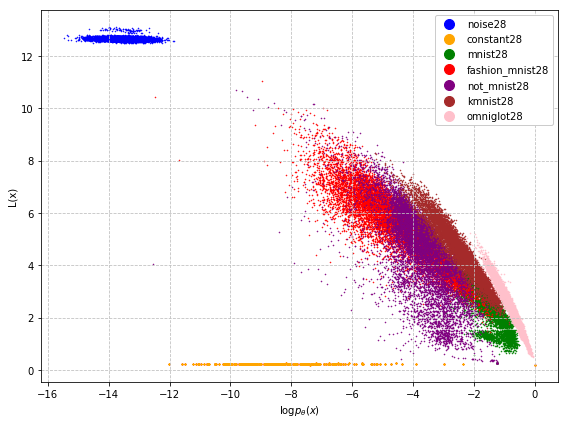
\includegraphics[width=0.45\columnwidth]{counterexample_complexity1}
}
\subfigure[AUROC = 0.9867]{
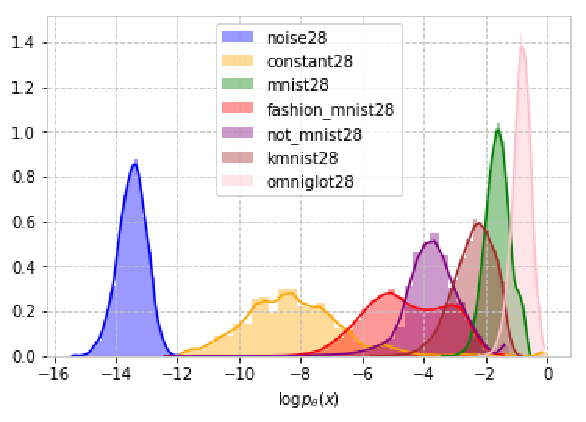
\includegraphics[width=0.45\columnwidth]{counterexample_complexity2}
}
\subfigure[AUROC = 0.7770]{
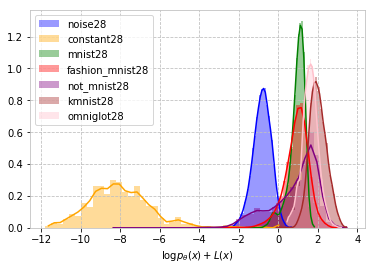
\includegraphics[width=0.45\columnwidth]{counterexample_complexity3}
}
\subfigure[AUROC = 0.9999]{
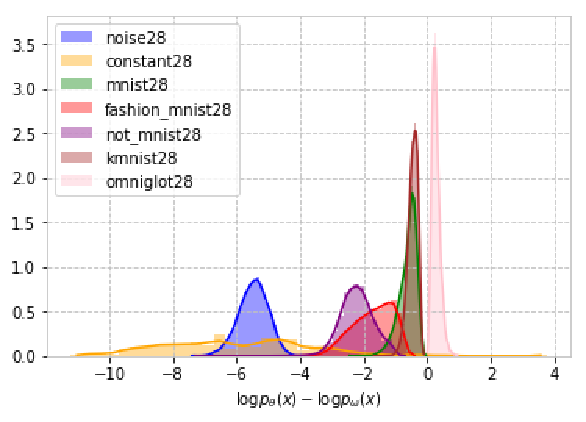
\includegraphics[width=0.45\columnwidth]{counterexample_complexity4}
}
\caption{We select Omniglot as in-distribution and other datasets as out-of-distribution. (a) shows the correlation between likelihoods trained on Omniglot and complexity estimate. (b) shows the histogram of log-likelihood, where the average AUROC is 0.9867. (c) shows that indicator $S(x)$ might reach lower the performance than log-likelihood. It means that $L(x)$ is rough and we need a more precise, stable and interpretable estimate to assist log-likelihood for detecting OoD. (d) shows $\log \frac{p_\theta(x)}{p_\omega(x)}$ might be a good choice where $p_\omega$ is trained on out-of-distribution.%(e) TODO shows that the density of samples on out-of-distribution increase instead decrease during training. 
}
\label{fig2}
\end{figure}

\subsection{Performance on Large-scale Datasets}

By following reasons, large-scale datasets is used to check the generality of indicators:

\noindent \textbf{1) Check observations} OoD indicators based on the motivating observation on few datasets, are unreliable. It is necessary to validate the generality of motivating observation. 

\noindent \textbf{2) Avoid over fine-tuning} The performance on few datasets might be easily improved by fine-tuning hyper-parameters and architectures of models, but hard on large-scale datasets. 

%\noindent \textbf{} By the definition of OoD problem in \Cref{sec2}, models should distinguish any $\pout$ that is distinct to $\pin$ instead of few datasets. Therefore, we should check more out-of-distribution as much as possible. 

\noindent \textbf{3) Average Performance} Average performance on large-scale datasets is better for assessing indicators. In CelebA vs LSUN, log-likelihood reaches 98\% AUROC, however, it only reaches 0.02 in CelebA vs SVHN in appendix A. Average performance will consider such experiments with lower AUROC. It is more meaningful to improve the average performance of indicators than to improve little (\EG 99.1\% to 99.2\%) in a single experiment. 

Indicators of previous works via common deep generative models do not perform well on large-scale datasets, as shown in \Cref{tab2}, where
DeConf-C, MCMC Recon, MCMC $\log p_\theta(x)$, $D_\theta(x)$, $\|\nabla_x D_\theta(x)\|$, entropy, $\max_{y} p(y|x)$, Mahalanobis, ODIN and disagreement are proposed by \cite{hendrycks2016baseline,hsu2020generalized,lee2018simple,alemi2018uncertainty,liang2018enhancing,kumar2019maximum,xu2018unsupervised,chen2019unsupervised,lakshminarayanan2017simple}. Perfect classifier is the classifier used to detect simply-classified, which is the theoretical optimal result. 
Thanking to the assistance of $L(x)$, $S(x)$ reaches the best performance among the past works, which encourages us to develop a better assistance in the next. 
%We observe that $\log p_\theta(x) - \log p_\omega(x)$ reaches outstanding performance near to theoretical optimal result on large-scale datasets. 

\begin{table}[t]
\centering
\begin{tabular}{lllllll}
indicator     & Model & AUROC & AUPR  \\
\toprule
Recon & VAE & 69.26 & 74.01 \\
% models/likelihood/vae.py --self_ood=True --count_experiment=True recon [0.69263249 0.74007645 0.48458715 0.74009771 0.41709495]
ELBO & VAE & 69.44 & 74.14 \\
% models/likelihood/vae.py --self_ood=True --count_experiment=True elbo [0.69441086 0.74140808 0.48346829 0.74142871 0.41541565]
ELBO - Recon & VAE & 52.85 & 58.93 \\
% models/likelihood/vae.py --self_ood=True --count_experiment=True elbo-recon [0.52854943 0.58930298 0.54053476 0.58945442 0.79552599]
MCMC Recon & VAE & 67.43 & 71.25 \\
% models/likelihood/vae.py --self_ood=True --count_experiment=True mcmc_recon [0.67433823 0.71252423 0.47690908 0.71255208 0.50583125]
MCMC $\log p_\theta(x)$ & VAE & 67.45 & 71.36 \\
% models/likelihood/vae.py --self_ood=True --count_experiment=True mcmc_ll [0.67449545 0.71361441 0.47851411 0.71364063 0.5008428 ]
Volume & RNVP & 62.46 & 70.63 \\
% models/likelihood/glow.py --self_ood=True --count_experiment=True log_det [0.62457946 0.70631498 0.52599346 0.7063359  0.50536926]
$\log p_\theta(z)$ & RNVP & 74.58 & 77.33 \\
% models/likelihood/glow.py --self_ood=True --count_experiment=True origin_log_prob [0.74578213 0.77333517 0.45129061 0.77335535 0.37895365]
H & VIB & 66.79 & 67.17 \\
% models/likelihood/vib.py --count_experiment=True nH [0.66791859 0.67165405 0.42322066 0.67171274 0.72936084]
R & VIB & 58.78 & 62.36 \\
% models/likelihood/vib.py --count_experiment=True R [0.58777827 0.62363702 0.43649377 0.6237109  0.81593815]
$D_\theta(x)$ & WGAN & 79.15 & 82.54 \\
$\|\nabla_x D_\theta(x)\|$ & WGAN & 60.55 & 65.14 \\
Disagreement & ResNet & 69.25 & 69.75\\
Mahalanobis & ResNet & 83.02 & 82.42 \\
Entropy of $p(y|x)$ & ResNet & 62.74 & 62.95 \\
$\max_{y} p(y|x)$ & ResNet & 61.59 & 64.90 \\
ODIN & ResNet & 60.68 & 60.98\\
% models/conditional/odin.py --count_experiment=True max_prob
DeConf-C & ResNet & 68.59 & 71.81 \\
% models/conditional/generalized_odin.py --count_experiment=True deconf_h [0.68586874 0.71805628 0.41233515 0.71370533 0.72274749]
DeConf-C* & ResNet & 71.09 & 73.92 \\
% models/conditional/generalized_odin.py --count_experiment=True deconf_h_hat_0.01 [0.71089042 0.73918372 0.40347142 0.73468261 0.64722223]classify & ResNet & 99.85 & 99.87 \\
Perfect classifier & ResNet & 99.85 & 99.87 \\
% models/conditional/pure_classifier.py --count_experiment=True classify [0.99847331 0.99868608 0.24623844 0.99738137 0.0123297 ]
\bottomrule
\bottomrule
\end{tabular}
\centering
\begin{tabular}{lllllll}
indicator     & VAE & PixelCNN & RNVP  \\
\toprule
$\log p_\theta(x)$ & 70.11 & 72.26 & 69.19 \\
% models/likelihood/vae.py --use_transductive=False --count_experiment=True log_prob [0.70112424 0.74344034 0.43742542 0.74346061 0.44621739]
$T_{perm}(x)$ & 89.71 & 84.28 & 89.72 \\
% models/likelihood/vae.py --self_ood=True --count_experiment=True T_perm [0.89705577 0.88169592 0.30420595 0.8817089  0.25626675]
$\|\nabla_x \log p_\theta(x)\|$ & 53.95 & NA & 24.27 \\
% models/likelihood/vae.py --self_ood=True --count_experiment=True grad_norm [0.53945138 0.58925883 0.53859666 0.58930938 0.75082352]
$S(x)$ & 81.88 & 88.33 & 80.11\\
% models/likelihood/vae.py --self_ood=True --count_experiment=True ll_with_complexity [0.8188339  0.85205757 0.39642634 0.85207535 0.34515788]
$LLR(x)$ & 69.47 & 77.46 & 64.03\\
% models/likelihood/vae.py --self_ood=True --count_experiment=True kl [0.69468958 0.69256431 0.48744052 0.69265109 0.50438847]
$WAIC(x)$ & 74.59 & 82.19 & 83.74 \\
% models/ensemble/vae.py --count_experiment=True ll_waic [0.74591325 0.77289253 0.44069799 0.77291618 0.4791148 ]
$\mathop{Var}_\theta [\log p_\theta(x)]$ & 83.11 & 82.21 & 86.06 \\
% models/ensemble/vae.py --count_experiment=True var_log_prob [0.83107434 0.84435032 0.35992672 0.84437826 0.38207751]
$\log p(x|y)$ & 53.13 & 69.22 & 71.27\\
% models/conditional/vae.py --count_experiment=True log_prob [0.53128465 0.56558425 0.54073484 0.56570161 0.81853378]
$T_{b, r_1, r_2}(x)$ & 67.26 & 56.98 & 77.38 \\
% models/batch_norm/vae.py --count_experiment=True r1_r2_log_pro [0.46404548 0.52311411 0.58300184 0.52327414 0.80378873]
$\log p_\theta(x)$ with BN & 85.15 & 64.10 & 82.00 \\
% models/batch_norm/vae.py --count_experiment=True log_prob_with_batch_norm [0.85145065 0.86582385 0.39921489 0.86583243 0.18485225]
$\log \frac{p_\theta(x)}{p_\omega(x)}$ & \textbf{99.08} & \textbf{99.85} & \textbf{99.81} \\
\bottomrule
\end{tabular}
\caption{Top table shows the average AUROC and AUPR of other past works on large-scale datasets. Bottom table shows the average AUROC of past works on large-scale datasets. $\log \frac{p_\theta(x)}{p_\omega(x)}$ is always outstanding, where $\omega$ is trained on OoD. 
}
\label{tab2}
\end{table}

\subsection{Observation of KL indicator}
As shown in \Cref{fig2}, complexity estimate is unstable and sometimes it might lower the performance. Therefore, we try to find another function to replace $L(x)$ in $S(x)$. 
In experiments on large-scale datasets, we observe a common phenomenon that $p_\theta(x) < p_\omega(x)$ for almost $x \sim \pout$ and $p_\theta(x) > p_\omega(x)$ for almost $x \sim \pin$ where $p_\omega(x)$ is a likelihood-based model trained on out-of-distribution. 
The average AUROC of $\log p_\theta(x) - \log p_\omega(x)$ reaches nearly 100\% on all datasets in \Cref{tab2}.
From the view of complexity estimate, $L(x) = -\log_2 p(x|\mathcal{M}_0)$ is the log-likelihood of a universal model $\mathcal{M}_0$~\cite{serra2019input}. In our paper, $p_\omega(x)$ is used to replace $L(x)$ to assist log-likelihood. 

However, in OoD problem, the out-of-distribution is not known. 
Therefore, we will explore how to develop an indicator that are not dependent on OoD and why $ \log \frac{p_\theta(x)}{p_\omega(x)}$ is almost useful for OoD theoretically. 

\section{Theorem}\label{sec5}
\subsection{Divergence-based Indicators}
%In the definition of OoD problem, we do not give any assumption about the probability distribution, since we try to make the definition more general. 
Our theory are based on following assumptions, which are also observed in experiments:

\noindent \textbf{1.} The training data and testing data of in-distribution and out-of-distribution are i.i.d. .

\noindent \textbf{2.}  $div$ is a divergence , satisfying that $div(\pin, \pout) \gg 0$ and $div(\pout, \pin) \gg 0$. 

\noindent \textbf{3.}  If $div(\pin, \pout)$ and $div(\pout, \pin)$ can be represented by sampling formula, \IE $div(\pin, \pout) \approx \sum_{i} f(x_i)$, then $f(x_i) \gg 0$ for almost $x_i$ in $\pin$. 

\noindent \textbf{4.} $f: \mathcal{X} \rightarrow \mathcal{R}$ maps the distribution $\pin, \pout$ into two Gaussian distribution with constant variance. 

\noindent \textbf{5.} Assumption 3 and 4 hold for any $\hat{f}$ approximating $f$. 


It is important to notice that assumption 3 can not be deduced from assumption 2 obviously. For example, when $\pin = \frac{1}{2}(\mathcal{N}(0, 1) + \mathcal{N}(-10, 1))$ and $\pout = \frac{1}{2}(\mathcal{N}(0, 1) + \mathcal{N}(10, 1))$, $KL(\pin, \pout) \approx 25.05 \gg 0$ but $\log \pin(x) - \log \pout(x) \approx 0$ for $x$ near 0.  In such example, $\pin$ and $\pout$ is distinguishing by KL-divergence but is not simply classified because no classifier can detect whether a sample in $[-1, 1]$ is from $\pin$ or $\pout$. We assume that assumption 3 holds when $\pin$ and $\pout$ is simply classified. 

The above assumptions mean that if $div$ can distinguishing the probability distribution                                                                                                        in-distribution and out-of-distribution, then $f$ can be used as an indicator for detecting whether a sample is OoD. $f$ is called the $div$-based indicator. 

For detailed research, \EG how to obtain indicators without knowing OoD, we need detailed property of $div$. 
In the next, we will introduce two concrete divergence-based indicators: KL-based indicator and Wasserstein-based indicator. 

\subsection{KL-based Indicator}
We choose KL-divergence as $div$, then $KL(\pin, \pout) = \E_{\pin(x)} [\log \pin(x) - \log \pout(x)]$ and KL-based indicator is $\log \pin(x) - \log \pout(x)$, whose motivation is in \Cref{fig3}. 

\begin{figure}[t]
	\centering
	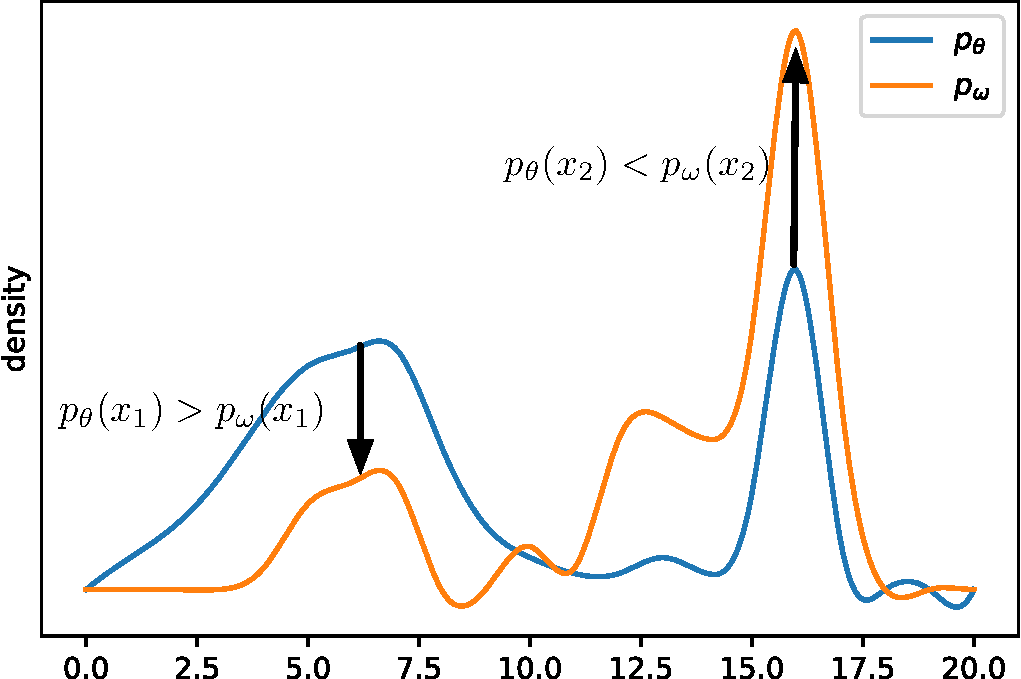
\includegraphics[width=0.8\columnwidth]{diagram.pdf}
	\caption{Diagrammatic sketch for KL-based indicator. The in-distribution is in [0, 10] and out-of-distribution in [10, 20]. Intuitively, $\pin$ assign lower density to samples from in-distribution and higher density for samples from out-of-distribution than $\pout$ . 
	Different to the assumption of likelihood indicator, we do not assume that $p_\theta(x_2)$ very small for $x_2 \sim \pout$. By the assumptions in \Cref{sec5}, we can induce that $p_\theta(x_1) > p_\omega(x_1)$ and $p_\theta(x_2) < p_\omega(x_2)$. Thus $\log p_\theta(x) - \log p_\omega(x)$ is an indicator for OoD detection. }
	\label{fig3}
\end{figure}

\begin{theorem}\label{thm1}
	$\log \pin(x) - \log \pout(x)$ is a symmetric indicator with great performance, \IE it reaches same performance in experiment A vs B and B vs A, with threshold zero. 
\end{theorem}
Likelihood is not a symmetric indicator since it uses $p_A$ as indicator in experiment A vs B and $p_B$ as indicator in experiment B vs A. An interesting phenomenon is that if likelihood indicator reaches a good performance on experiment A vs B, it will usually fail in experiment B vs A, in appendix B. Especially, in experiments of Noise vs any dataset, the optimal model for Noise dataset is uniform distribution, but it can not detect any OoD. In the experiment of any dataset vs Noise, likelihood reaches nearly 100\% AUROC since the likelihood of noise is significantly lower than any datasets. 

However, $\pout$ is unknown in the OoD problem. Therefore, we try to use another tractable term to replace $\pout$. 

\begin{theorem}\label{thm2}
	For any mixture distribution $\pmix = \alpha \pin + \beta \pout$ where $\alpha + \beta = 1$ and $\alpha, \beta > 0$, the performance of indicator $\log \pin(x) - \log \pmix(x)$ and indicator $\log \pin(x) - \log \pout(x)$ is equal for OoD detection. 
\end{theorem}

If we can get enough data from the mixture distribution, by \Cref{thm1}, $\pmix$ can be used to replace the term $\pout$ in KL-based indicator and keep the same performance, which is shown in experiments in \Cref{tab3}. Next, we try to explain why KL-based indicator can reach outstanding performance.

Compared to likelihood indicator and likelihood-ratio indicator, KL-based indicator can get better performance. 
\begin{theorem}\label{thm3}
When log-likelihood can detect OoD, \IE $\log \pin(x_1) > \log \pin(x_2)$ for almost $x_1 \sim \pin$ and $x_2 \sim \pout$, KL-based indicator can be also used to detect OoD. 
\end{theorem}

\begin{theorem}\label{thm4}
For any likelihood-ratio indicator $\log \pin(x) - \log g(x)$ where $g$ is a continuous differentiable probability distribution, KL-based indicator outperforms them. 
\end{theorem}

Above theorems show that $\log \frac{\pin(x)}{\pmix(x)}$ is a good OoD indicator. It is a natural idea to model in-distribution and mixture distribution by $p_\theta, p_\gamma$, \IE $\max_\theta \E_{\pin(x)} \log p_\theta(x)$ and $\max_\gamma \E_{\pmix(x)} \log p_\gamma(x)$ are used as loss to train model. 
Next, we will show the property of model distribution. 

\begin{theorem}\label{thm5}
	$\log \frac{p_\theta(x)}{p_\gamma(x)}$ can be used for detecting OoD. Moreover, $\log \frac{p_\theta(x)}{p_\gamma(x)}$ represents whether a sample $x$ in mixture distribution have been optimized in the training process of $\theta$. 
\end{theorem}

\Cref{thm5} shows that $\log \frac{p_\theta(x)}{p_\gamma(x)}$ represents the optimizability: if a sample $x$ is OoD, $p_\theta(x)$ will be lower than $p_\gamma(x)$ since $x$ is also in $\pmix$ and $p_\gamma(x)$ can be optimized more than $p_\theta(x)$; if $x$ is not OoD, $p_\theta(x)$ will not be lower than $p_\gamma(x)$ since $p_\theta(x)$ is well-trained to maximize log-likelihood. \Cref{thm5} indicates that we do not need spend much time for training on mixture distribution since we only need to observe whether the likelihood of a sample can be improved, which can be shown in few epochs. It alleviates the requirements for training and then we can train models online. 

\subsection{Wasserstein-based Indicator}
From the view of traditional likelihood-indicator, GANs can not be used for detecting OoD since  how to evaluate the density of GANs is an open problem\cite{nalisnick2019do}. Therefore, some researches propose variants of GANs with tractable density~\cite{kumar2019maximum}. In the framework of divergence-based indicators, we can detect OoD by discriminator without the density of GANs.                                                                                                                                                                                                                                                                                                                                                                                                      

In vanilla GAN~\cite{goodfellow2014generative}, a discriminator is trained to distinguish generated samples and real samples and  a generator is trained to generate samples for deceiving the discriminator.

However, vanilla GAN is unstable during the training process. To tackle this problem, Wasserstein distance is introduced by WGAN~\cite{arjovsky2017wasserstein}:
\begin{equation}
	W^1(\mu, \nu) = \sup_{Lip(D) \leq 1} \{\E_{\mu(x)} D(x)  - \E_{\nu(x)} D(x)\}
\end{equation}

We select Wasserstein distance as $div$, then
\begin{equation}
	W^1(\pin, \pout) \approx \sum_i \Big[D(x_i^{in}) - \sum_j D(x_j^{out})\Big]
\end{equation} 
where $x_i^{in}$ is sampled from in-distribution, $x_j^{out}$ is sampled from out-of-distribution and $D$ is the optimal solution in $W^1(\pin, \pout)$. Then the Wasserstein-based indicator for sample $x$ is $D(x) - \sum_{j} D(x_j^{out})$. Notice that $\sum_{j} D(x_j^{out})$ is a constant and it will not affect the performance of OoD detection. Therefore, the Wasserstein-based indicator is simply $D(x)$. The generator of WGAN does not appear in our formula since we only consider how to measure the distance between $\pin, \pout$ instead of generating. 

We will show some theorems to show the property of Wasserstein-based indicator to ensure that it can be obtained without any information of $\pout$. 

\begin{theorem}\label{thm6}
	Assumption 2 is a corollary of definition of OoD problem when $div$ is Wasserstein distance.  
\end{theorem}

\begin{theorem}\label{thm7}
	$D(x)$ is a symmetric indicator. 
\end{theorem}

\begin{theorem}\label{thm8}
	$\hat{D}$ that is optimal solution in $W^1(\pin, \pmix)$ is same to the optimal solution $D$ in $W^1(\pin, \pout)$. Moreover, the neural networks trained by $W^1(\pin, \pmix)$ and $W^1(\pin, \pout)$ will share the same optimization process. 
\end{theorem}

By \Cref{thm8}, $\hat{D}$ that is easy-obtained can replace $D$. Next theorem will ensure the performance of it. 

\begin{theorem}\label{thm9}
	The discriminator in $W^1(\pin, \pout)$ is the best indicator among all indicators that is 1-Lipschitz. Moreover, it is the best indicator who has limited gradient. 
\end{theorem}

\subsection{Concerns}
We have proposed a method to exploit the samples of mixture distribution to train a model for OoD detection. However, there are three major concerns about this idea: 

\noindent \textbf{1.} Is our method \textbf{data-specific}? \IE does this method only work on the data that it has seen in training? 

\noindent \textbf{2.} Can our method work \textbf{online}? \IE for new testing data, indicators should be given before the next testing data come.  

\noindent \textbf{3.} Can our method work on a \textbf{small size block} while model must detect OoD immediately while it only knows in-distribution data and this block from mixture distribution. 

\noindent \textbf{4.} Is it better to train \textbf{pre-trained} models (trained on in-distribution) or \textbf{initialized} models on mixture distribution?

To solve the concerns, we design following experiments:

\noindent \textbf{1.} In experiment A vs B, only 20\% data in mixture distribution can be used for training. 

\noindent \textbf{2.} We simulate the online system --- the data in mixture distribution is streaming and requires indicators immediately. 

\noindent \textbf{3.} We splits the data from mixture distribution into several blocks and model can only be trained on the in-distribution and the block waiting for detection.  

\noindent \textbf{4.} Experiments for pre-train models and initialized models. 

\section{Experiments}\label{sec6}
In this section, we will demonstrate the effectiveness of KL-based indicator and Wasserstein-based indicator on large-scale computer vision benchmark datasets. 
%We run all experiments with Pytorch and Tensorflow and we submit the code to reproduce all experimental results. 

\subsection{Datasets}
%All the datasets considered are listed below:
%\textbf{CIFAR-10}~\cite{krizhevsky2009learning} is a natural image datasets with 10 classes including animal, ship, airplane and etc. 
%\textbf{CIFAR-100}~\cite{krizhevsky2009learning} is just like CIFAR-10, including 100 classes. 
%\textbf{SVHN}~\cite{netzer2011reading} includes house numbers from 0 to 9. 
%\textbf{CelebA}~\cite{liu2015deep} is a large-scale face attributes dataset. 
%\textbf{TinyImageNet} consists of a subset of ImageNet images. It contains 200 different classes.
%\textbf{LSUN} has a testing set of 10 different scenes. 
%\textbf{iSUN} is subset of SUN, including 8925 scene images in 899 different scenes.
%\textbf{MNIST} consists of handwritten digits from 0 to 9. 
%\textbf{Fashion MNIST} includes 10 kinds of clothes and shoes. 
%\textbf{Not MNIST} includes letters from A to J on various typefaces. 
%\textbf{KMNIST} includes 10 kinds of Kanji characters.
%\textbf{Omniglot} contains 1623 different handwritten characters from 50 different alphabets. 
%\textbf{Noise} is created by uniformly randomly sampling. 
%\textbf{Constant} includes images whose pixels have same color. 

MNIST~\cite{lecun1998gradient-based}, FashionMNIST~\cite{xiao2017/online}, KMNIST~\cite{clanuwat2018deep}, NOT-MNIST, Omniglot~\cite{lake2015human}, CIFAR-10~\cite{krizhevsky2009learning}, CIFAR-100~\cite{krizhevsky2009learning}, TinyImagenet~\cite{deng2009imagenet}, SVHN~\cite{netzer2011reading}, iSUN~\cite{xu2015turkergaze}, CelebA~\cite{liu2015deep}, LSUN~\cite{yu2015lsun}, Noise and Constant are considered. 

The natural images are resized into 32x32x3 and grey images are all 28x28x1. All pair in natural image datasets and all pair in grey image datasets are considered in our experiments. Only CIFAR-10, CIFAR-100 and TinyImageNet are not simply-classified and intuitively they have similar classes. Noise and Constant includes both grey and natural images. LSUN and iSUN are only used for out-of-distribution. CelebA, Noise and Constant have no labels, and we set random labels from 0 to 9 on these datasets. 

Samples of $\pin, \pout$ are from training set of $\pin, \pout$. Samples of $\pmix$ are from the testing set of $\pin, \pout$. 

\subsection{Metrics}
Following metrics are adopted to measure the effectiveness of a method in out-of-distribution detection:

\noindent \textbf{AUROC} is the Area Under the Receiver Operating Characteristic curve, which is a threshold-independent metric~\cite{davis2006relationship}. AUROC can be interpreted as the probability that a sample from in-distribution is assigned a lower detection score than a sample from out-of-distribution~\cite{fawcett2006introduction}. It is widely applied in OoD domain. We select AUROC as our major metrics. 


\noindent \textbf{AP} is the Average Precision, summarizing the precision-recall curve as the weighted mean of precisions achieved at each threshold. 

\noindent \textbf{FPR@TPR95} is the False Positive Rate when True Positive Rate is over 95\%., which means the probability that an out-of-distribution example is misclassified as in-distribution when over 95\% in-distribution is detected accurately.

\noindent \textbf{AUPR} is the Area under the Precision-Recall curve, which is also threshold independent~\cite{saito2015precision}. % AUPR-In and AUPR-Out denotes the AUPR where in-distribution and out-of-distribution are positive, respectively.  


\subsection{Setups} 
For fair comparison, all indicators are based on common models with standard training, including 34-layer ResNet, VAE, PixelCNN, RealNVP and Wasserstein GAN. ResNet34 is trained for classification and serves for the OoD indicators based on classifier. ResNet34 is also trained to classify in-distribution and out-of-distribution for validating whether they are simply classified. Deep generative models are trained as their proposers suggest. 

In our experiments, there is no validation set. For indicators depending on hyper-parameters, we try grid-searching as their proposers suggest and report the performance with all hyper-parameters considered. To ensure the generality on all datasets, it is forbidden to specify the hyper-parameters or architectures on special dataset. 
The detailed architecture and parameters are shown in appendix B. 

\subsection{Major Results}


\begin{table}[htbp]
\centering
\begin{tabular}{lllllll}
indicator     & Model & AUROC & AUPR  \\
\toprule
$\log \frac{p_\theta(x)}{p_\omega(x)}$ & VAE & 99.08 & 99.03 \\
% models/likelihood/vae.py --use_transductive=False --count_experiment=True kl [0.99084057 0.99026414 0.30887569 0.99026842 0.01531516]
$\log \frac{p_\theta(x)}{p_\omega(x)}$ & PixelCNN & 99.85 & 99.82 \\
% models/likelihood/pixelcnn.py --use_transductive=False --count_experiment=True kl [0.9985365  0.99822038 0.30394854 0.9982208  0.00421367]
$\log \frac{p_\theta(x)}{p_\omega(x)}$ & RNVP & 99.81 & 99.77 \\
% models/likelihood/glow.py --use_transductive=False --count_experiment=True kl [0.99814327 0.99774027 0.30394204 0.99774489 0.0071557 ]
$D_\omega(x)$ & WGAN & 98.57 & 98.40 \\
% models/wgan/wasserstein.py --use_transductive=False --count_experiment=True log_prob [0.98574477 0.98397579 0.30537663 0.98398171 0.05851498]
$\log \frac{p_\theta(x)}{p_\gamma(x)}$ & VAE & 98.44 & 98.31 \\
% models/likelihood/vae.py --count_experiment=True kl [0.9844299  0.98307137 0.31120329 0.98307722 0.02728208]
$\log \frac{p_\theta(x)}{p_\gamma(x)}$ & PixelCNN & 97.23 & 95.91 \\
% models/likelihood/pixelcnn.py --count_experiment=True kl [0.97226134 0.9590684  0.31843328 0.95907839 0.04293366]
$\log \frac{p_\theta(x)}{p_\gamma(x)}$ & RNVP & 97.99 & 97.40 \\
% models/likelihood/glow.py --count_experiment=True kl [0.97990943 0.97399013 0.3090165  0.97400243 0.05367133]
$D_\gamma(x)$  & WGAN & 98.06 & 98.20 \\
% models/wgan/wasserstein.py --count_experiment=True log_prob [0.98060671 0.98203186 0.30591395 0.98203785 0.08610534]
\bottomrule
\end{tabular}
\caption{The performance of divergence-based Indicators. $\gamma, \omega$ are trained on $\pmix$ and $\pout$ respectively. }
\label{tab3}
\end{table}

The main results for indicators of past works are summarized in \Cref{tab2}. The main results for KL-based indicator and Wasserstein-based indicator are summarized in \Cref{tab3}. 

\subsection{Validation of Theorem}

\Cref{thm1} is supported by the detail experiments shown in appendix B. \Cref{thm2} is supported by \Cref{tab3}, where the performance of $\log \frac{p_\theta(x)}{p_\gamma(x)}$ is nearly same as $\log \frac{p_\theta(x)}{p_\omega(x)}$. 

Detailed experiments in appendix B show that KL-based indicator can get same performance when log-likelihood can reach outstanding performance, to support \Cref{thm3}. 

\begin{figure}[t]
	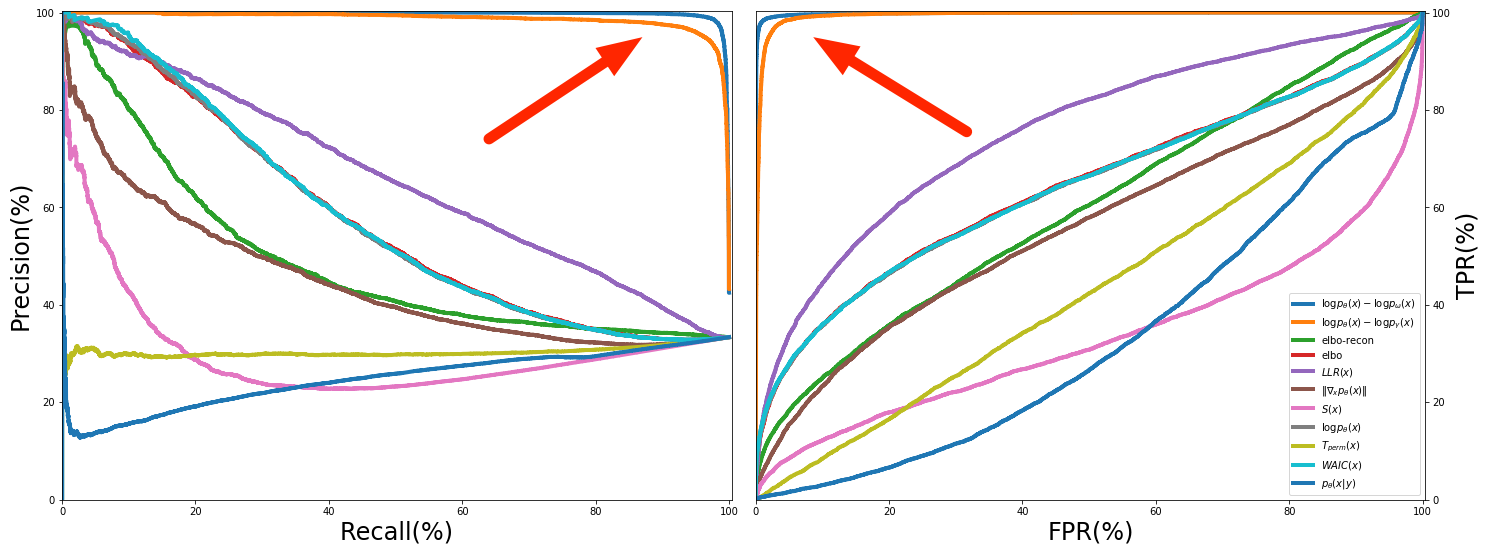
\includegraphics[width=0.9\columnwidth]{roc_prc}
	\caption{ROC and PRC on CIFAR-100 vs CelebA based on VAE model. The KL-based indicator outperforms others. }
	\label{fig5}
\end{figure}

We compare the precision-recall curve and ROC curve of KL-based indicator, log-likelihood indicator, likelihood ratio indicator and log-likelihood with input complexity in \Cref{fig5}, to show KL-based indicator is the best version of log-likelihood ratio indicator, to support \Cref{thm4}. 

\Cref{thm7} is supported by the detailed experiments in appendix B. In \Cref{tab3}, the performance of $D_\omega(x)$ is nearly same as $D_\gamma(x)$, which supports \Cref{thm8}. The outstanding performance of $D_\omega(x), D_\gamma(x)$ supports the \Cref{thm9}. 

\subsection{Concerns}
\begin{table}[htbp]
\centering
\begin{tabular}{lllllll}
Limit & indicator  & Model & AUROC & AUPR  \\
\toprule
online & $\log \frac{p_\theta(x)}{p_\gamma(x)}$ & VAE & 97.24 & 95.92 \\
% models/increment/vae.py --count_experiment=True kl [0.97243253 0.95917428 0.30967758 0.95918684 0.07459903]
online & $\log \frac{p_\theta(x)}{p_\gamma(x)}$ & PixelCNN & 91.77 & 90.14 \\
% models/increment/pixelcnn.py --count_experiment=True kl [0.91768834 0.90141178 0.34569425 0.90142671 0.13461902]
online & $\log \frac{p_\theta(x)}{p_\gamma(x)}$ & RNVP & 90.92 & 90.89 \\
% models/increment/glow.py --count_experiment=True kl [0.90919486 0.90890549 0.33934175 0.90892716 0.17370991]
online & $D_\gamma(x)$ & WGAN & 97.96 & 98.16 \\
% models/increment/wasserstein.py --count_experiment=True kl [0.97961287 0.98159097 0.30585588 0.98159486 0.09025942]
20\% & $\log \frac{p_\theta(x)}{p_\theta(x)}$ & VAE & 96.50 & 94.97 \\
% models/likelihood/vae.py --mixed_ratio=0.2 --count_experiment=True kl [0.96503215 0.94974976 0.31624716 0.94976225 0.07812461]
20\% & $\log \frac{p_\theta(x)}{p_\gamma(x)}$ & PixelCNN & 91.47 & 90.83 \\
% models/likelihood/pixelcnn.py --mixed_ratio=0.2 --count_experiment=True kl [0.91468939 0.90826535 0.35387375 0.90827948 0.1352672 ]
20\% & $\log \frac{p_\theta(x)}{p_\gamma(x)}$ & RNVP & 88.16 & 88.84 \\
% models/likelihood/glow.py --mixed_ratio=0.2 --count_experiment=True kl [0.88160592 0.88837725 0.35641642 0.88839901 0.20640805]
20\% & $D_\gamma(x)$ & WGAN & 98.09 & 98.22 \\
% models/wgan/wasserstein.py --mixed_ratio=0.2 --count_experiment=True log_prob [0.98092962 0.98222605 0.30582678 0.98223201 0.08401409]
block & $\log \frac{p_\theta(x)}{p_\gamma(x)}$ & VAE & 97.60 & 96.26 \\
% models/increment/vae.py --retrain_for_batch=True --count_experiment=True kl [0.97600015 0.96260617 0.30931733 0.96262074 0.07344461]
block & $\log \frac{p_\theta(x)}{p_\gamma(x)}$ & PixelCNN & 88.80 & 88.96 \\
% models/increment/pixelcnn.py --retrain_for_batch=True --count_experiment=True kl [0.8880322  0.88963066 0.36653479 0.88964384 0.16618982]
block & $\log \frac{p_\theta(x)}{p_\gamma(x)}$ & RNVP & 90.44 & 90.83 \\
% models/increment/glow.py --retrain_for_batch=True --count_experiment=True kl [0.90439109 0.90831302 0.34553127 0.90833221 0.16889964]
block & $D_\gamma(x)$ & WGAN & 97.66 & 97.89 \\
% models/increment/wasserstein.py --retrain_for_batch=True --count_experiment=True kl [0.97663634 0.97891633 0.30628251 0.97891805 0.10417664]
\bottomrule
\end{tabular}
\caption{The average online testing time (including training time on $\pout$) per image for VAE, PixelCNN, RNVP and WGAN is 0.18s, 0.13s, 0.58s and 0.11s. 'online' indicates that data is streaming, '20\%' indicates that only 20\% data in $\pmix$ can be used for training and 'block' indicates that only a block can be used. VAE and WGAN are more robust since their performance is near to the value in \cref{tab3}. }
\label{tab4}
\end{table}

\begin{figure}[t]
\centering
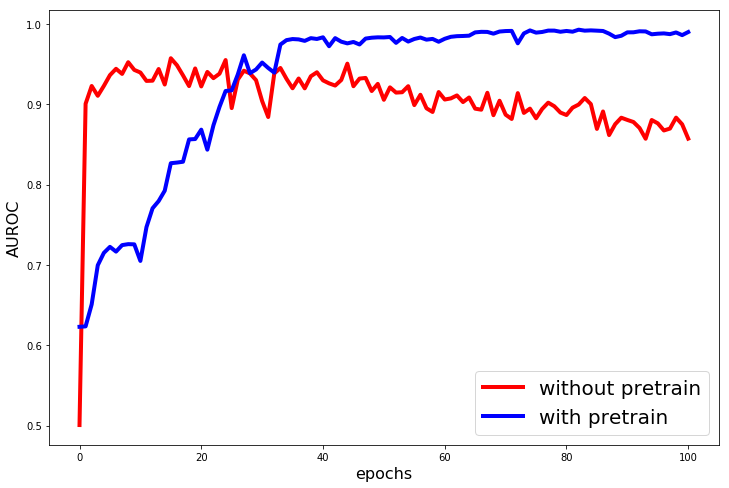
\includegraphics[width=0.45\columnwidth]{auroc_during_training}
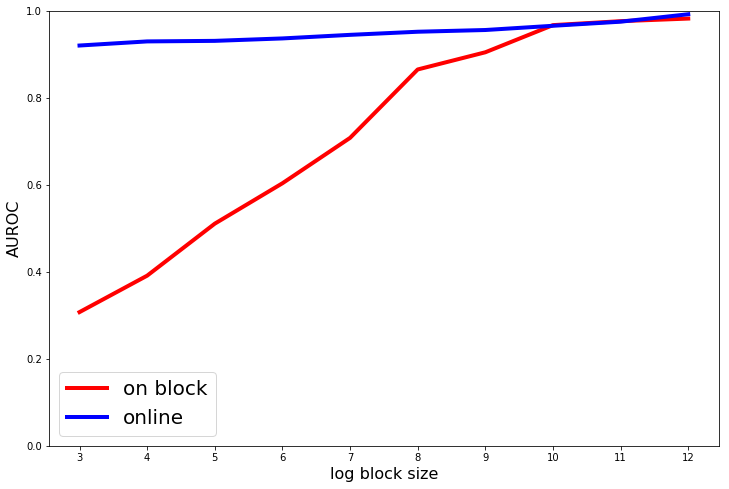
\includegraphics[width=0.45\columnwidth]{auroc_during_batch}
\caption{Left figure shows the changing of average AUROC of pretrained model and un-pretrained model during the training on $\pmix$, on CIFAR-10 vs other datasets. Pretrained model can easily get a good performance after few epochs, but it will fall into the local extremum (likelihood on in-distribution has been optimized quite well in pre-training, and any modification for parameters will reduce it) and the final performance is not well. Un-pretrained model need more epochs to get a good performance, but its final performance is better than pretrained model. 
Right figure shows the changing of AUROC of KL-based indicator when the block size varies on CIFAR-10 vs SVHN. It shows the limitation: when block size is small enough, the optimization only on one block will lead to unexpected $p_\gamma$. Training on past data (online) can alleviate this issue. Block size of 'online' means the size of data streaming at same time. }
\label{fig6}
\end{figure}

The experiments about concerns are showing in \Cref{tab4}. \Cref{fig6} shows the change of AUROC during training on $\pmix$. 
\Cref{fig6} shows the change of AUROC while the size of block varies. 
These experiments show that KL-based indicator and Wasserstein-based indicator are effective, robust, general, online and not data-specific. It also shows the weakness of that they can not work well in a small enough block. 

\subsection{Limitations of the Study} 
%In this section, we will discuss the limitation of our paper in datasets, models and divergence-based indicators. 

\noindent \textbf{Limitation of datasets.}
In our paper, we use large-scale datasets to show the generality of indicators. However, we only consider natural OoD datasets and do not consider attacked OoD, which are categorized by \cite{chen2020robust}. An important reason is that there is not a universal principle like simply classified, to measure these attacked OoD datasets. 

\noindent \textbf{Limitation of models.} 
In our paper, for fair comparison and generality, we only consider the common models, including ResNet, VAE, PixelCNN, RealNVP and WGAN. However, there are numerous models careful-designed for OoD detection. Due to the resource limitation, we can not give the performance of them on large-scale datasets. We emphasize that evaluation in a few datasets is unreliable and we expect that it can become a common sense in the OoD domain. 

\noindent \textbf{Limitation of divergence-based indicators.} 
Some defects of divergence-based indicators is shown, while they reach outstanding performance. They rely on the model (\EG KL-based indicator on RNVP is more data-specific) and optimizer (\EG when data from mixture distribution is not enough for training, optimizer can not give the expected $p_\gamma$). It is a natural idea to approximate $\log \frac{ p_\theta(x)}{p_\gamma(x)}$ without optimizer, \EG Taylor Expansion on pretrained model. We leave it for future work. 
Divergence-based indicators will guide future works since it can develop simply, fundamental and practical indicators from basic assumptions. 

\section{Conclusion and Future Work}
In this paper, we show the terrible generality of existing OoD indicators based on common models on large-scale datasets and call on that evaluation on large-scale datasets is crucial in OoD domain. We propose the KL-based indicator and the Wasserstein-based indicator through the divergence-based indicator theoretical framework, which is a novel idea that can guide OoD indicators based on deep generative models. Our indicators achieve the state-of-the-art on large-scale datasets, outperforming past works by 10\% in AUROC.

For future work, it will be interesting to approximate KL-based indicator without optimizer or develop optimizers that only require few data to train models on mixture distribution, for solving the limitation of divergence-based indicators.  We believe our paper will provide insight into the development of OoD indicators based on deep generative models. 

\newpage
\section{Ethical and societal impact}
There is no any potential ethical impact of our work. Our work focus on pure model research. The datasets and model considered in our paper are open, clear and popular. Our work concentrate on developing new OoD detector based on deep generative models, which might play important role in anomaly detection or assisting the classification. Our paper does not have any negative societal implications.  
\bibliography{reference.bib}

\end{document}
